\documentclass[10pt, a5paper]{article}
\usepackage{pdfpages}
\usepackage{parallel}
\usepackage[T2A]{fontenc}
\usepackage{ucs}
\usepackage[utf8x]{inputenc}
\usepackage[polish,english,russian]{babel}
\usepackage{hyperref}
\usepackage{rotating}
\usepackage[inner=2cm,top=1.8cm,outer=2cm,bottom=2.3cm,nohead]{geometry}
\usepackage{listings}
\usepackage{graphicx}
\usepackage{wrapfig}
\usepackage{longtable}
\usepackage{indentfirst}
\usepackage{array}
\newcolumntype{P}[1]{>{\raggedright\arraybackslash}p{#1}}
\frenchspacing
\usepackage{fixltx2e} %text sub- and superscripts
\usepackage{icomma} % коскі ў матэматычным рэжыме
\PreloadUnicodePage{4}

\newcommand{\longpage}{\enlargethispage{\baselineskip}}
\newcommand{\shortpage}{\enlargethispage{-\baselineskip}}

\def\switchlang#1{\expandafter\csname switchlang#1\endcsname}
\def\switchlangbe{
\let\saverefname=\refname%
\def\refname{Літаратура}%
\def\figurename{Іл.}%
}
\def\switchlangen{
\let\saverefname=\refname%
\def\refname{References}%
\def\figurename{Fig.}%
}
\def\switchlangru{
\let\saverefname=\refname%
\let\savefigurename=\figurename%
\def\refname{Литература}%
\def\figurename{Рис.}%
}

\hyphenation{admi-ni-stra-tive}
\hyphenation{ex-pe-ri-ence}
\hyphenation{fle-xi-bi-li-ty}
\hyphenation{Py-thon}
\hyphenation{ma-the-ma-ti-cal}
\hyphenation{re-ported}
\hyphenation{imp-le-menta-tions}
\hyphenation{pro-vides}
\hyphenation{en-gi-neering}
\hyphenation{com-pa-ti-bi-li-ty}
\hyphenation{im-pos-sible}
\hyphenation{desk-top}
\hyphenation{elec-tro-nic}
\hyphenation{com-pa-ny}
\hyphenation{de-ve-lop-ment}
\hyphenation{de-ve-loping}
\hyphenation{de-ve-lop}
\hyphenation{da-ta-ba-se}
\hyphenation{plat-forms}
\hyphenation{or-ga-ni-za-tion}
\hyphenation{pro-gramming}
\hyphenation{in-stru-ments}
\hyphenation{Li-nux}
\hyphenation{sour-ce}
\hyphenation{en-vi-ron-ment}
\hyphenation{Te-le-pathy}
\hyphenation{Li-nux-ov-ka}
\hyphenation{Open-BSD}
\hyphenation{Free-BSD}
\hyphenation{men-ti-on-ed}
\hyphenation{app-li-ca-tion}

\def\progref!#1!{\texttt{#1}}
\renewcommand{\arraystretch}{2} %Іначай формулы ў матрыцы зліпаюцца з лініямі
\usepackage{array}

\def\interview #1 (#2), #3, #4, #5\par{

\section[#1, #3, #4]{#1 -- #3, #4}
\def\qname{LVEE}
\def\aname{#1}
\def\q ##1\par{{\noindent \bf \qname: ##1 }\par}
\def\a{{\noindent \bf \aname: } \def\qname{L}\def\aname{#2}}
}

\def\interview* #1 (#2), #3, #4, #5\par{

\section*{#1\\{\small\rm #3, #4. #5}}

\def\qname{LVEE}
\def\aname{#1}
\def\q ##1\par{{\noindent \bf \qname: ##1 }\par}
\def\a{{\noindent \bf \aname: } \def\qname{L}\def\aname{#2}}
}

\switchlang{en}
\begin{document}
\title{Software Generators of Petri Net Models}
\author{Tatiana R. Shmeleva, Odessa, Ukraine\footnote{\url{tishtri@rambler.ru}, \url {https://lvee.org/ru/abstracts/299}}}
\maketitle
\begin{abstract}
Petri net models of variable size having definite structure are characteristic for manifold application domains such as \linebreak networking and high performance computing, manufacturing \linebreak control, and structural biology. A formalism of infinite Petri nets allows us to specify suchlike systems. Though models of definite size are of some interest for illustrative purposes. Moreover, an inductive technique for drawing conclusions on an infinite model properties is based on a sequence of models with growing size. A technique of composing programs in C language which generate Petri net models is developed, a dozen of generators implemented and available via GitHub as open source software. Models are represented either in graphical format for 2D case or in logical format for higher number of dimensions. 
\end{abstract}
\subsection*{Introduction}

Communication grids find wide application in radio and cellular networks, numerical parallel solving tasks by the method of finite ele\-ments, as communication subsystems of supercomputers (especially, multidimensional torus), and network-on-chip structures. Petri net \linebreak models of communication grids are considered in \cite{bib1} and \cite{bib2}. To find their properties for verification of corresponging protocols and their performance evaluation, we need a collection of models having incremen\-ted size.

To avoid laborious work with manual editing bulky Petri net models of real-life objects having regular structure, our software generates models automatically on a given set of parameters.

Petri nets are a part of UML notation \cite{bib3} for specification of parallel processes. They find wide application as a language of parallel programming \cite{bib4}, for verification of parallel programs and networking \linebreak protocols \cite{bib1},\cite{bib2}, modeling automated manufacture \cite{bib5}, and in avionics \cite{bib6}.

Let us consider examples of triangular (fig. \ref{Shmeleva:fig1}) and  hexagonal switching grid structures (fig. \ref{Shmeleva:fig2}) of size 4 generated by the correspon\-ding programs studied in the present paper.

\begin{center}
\begin{figure}[h!]
  \centering
  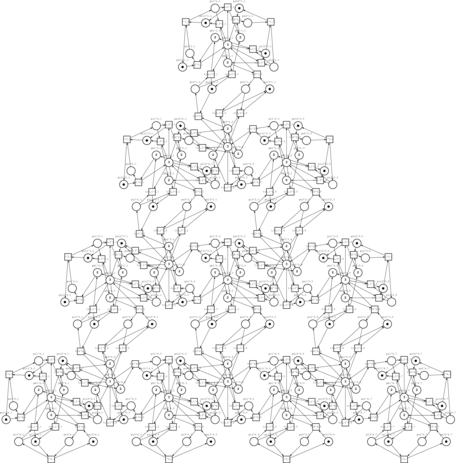
\includegraphics[width=8cm]{14_Shmeleva_fig1.png}
  \caption{~}
  \label{Shmeleva:fig1}
\end{figure}
\end{center}

\begin{center}
\begin{figure}[h!]
  \centering
  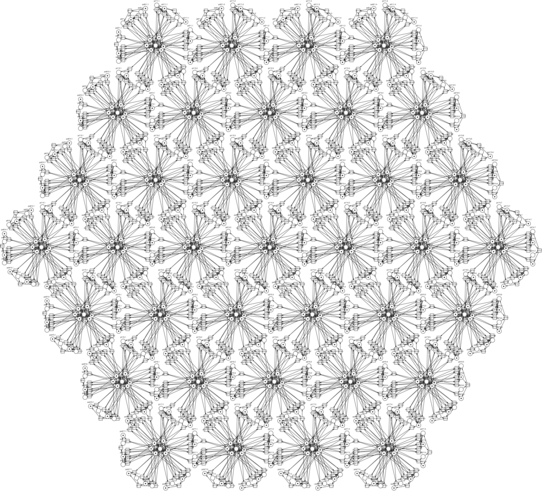
\includegraphics[width=8cm]{14_Shmeleva_fig2.png}
  \caption{~}
  \label{Shmeleva:fig2}
\end{figure}
\end{center}

An infinite Petri net is a powerful abstraction described in \cite{bib1} and \cite{bib2}, which allows the specification of models having an arbitrary size but a definite structure obtained by spatial composition of one or more basic components. An overwhelming result is obtained that gives a way to draw conclusions on properties of models with no regard to their size. For visualization and application of inductive methods which draw conclusions for infinite nets of definite structure, a fast facility that creates a model of a given size is required.

We developed a technique of software generators design based on the infinite Petri net specification and a series of about a dozen of generators of switching grid structure of square, triangular, and hexa\-gonal form on a plane (2D) as well as hypercube and hypertorus in multidimensional space listed in the Conclusions section. The open source software has been uploaded on GitHub and is compatible on data formats with modeling system Tina \cite{bib7}.

Modeling system Tina \cite{bib7} is for years de facto standard for Petri net models exchange and analysis; in 2019, Tina has won international Model Checking Contest. It allows automatic visualization of models, building its state space and finding structural properties \cite{bib5} as well as reflecting Petri net behavior --- token game.

\subsection*{Specification of Infinite Petri Nets}

The basic technique allows studying an infinite structures using their finite parametric specification obtained by repetition and composi\-tion of a single component. Our models are divided into two classes: for grids with definite number of dimensions, basically 1D and 2D; for grids with arbitrary number of dimensions. In the first case we use parameters of size only while in the second case a parameter which defines the number of dimensions is added. Structures having more than one basic component can be studied as well.

For majority of models we consider a cellular structure which implies connections of cells according to von Neumann neighborhood, some models are composed using Moore neighborhood, a generalized Zaitsev neighborhood is applied as well. Connection of neighbor cells is obtained by merging their contact places.

Remind that a Petri net is a bipartite directed graph supplied with dynamic elements called tokens. One part of vertices is called places and drawn as circles while the other part of vertices is called transitions and drawn as rectangles. We use notation of a parametric multiset rewriting system, each row specifies a transition by lists of its input and output places.

Let us consider a square grid specification obtained from a basic component represented by a single place as its repetition in cells of a two dimensional grid supplied by transitions according to von Neumann neighborhood written in TEX notation:

\begin{verbatim}
\begin{equation}\left(
\left(
\begin{array}{l}
t_{1,1}^{i,j}: p^{i,j} -> p^{i-1,j}, i>1,\\
t_{1,2}^{i,j}: p^{i,j} -> p^{i+1,j}, i<n,\\
t_{2,1}^{i,j}: p^{i,j} -> p^{i,j-1}, j>1,\\
t_{2,2}^{i,j}: p^{i,j} -> p^{i,j-1}, j<n,\\
\end{array}
\right),
1<=i<=n, 1<=j<=n, 
\right)
\end{equation}.\end{verbatim}
The parameter n gives the grid size while variables i and j specify the cell indices in horizontal and vertical directions correspondingly. The upper index (i,j) gives the cell location inside the lattice; i goes from top to down and j goes from left to right. Enumeration of transitions using two lower indices (d,r) suits multidimensional grid as well; d gives the number of dimension and r gives one of two directions: 1 -- to the origin, 2 -- to infinity.

\subsection*{Generators of Models in Logical Format}

Models in logical format are rather simple specifying names of places and transitions and their connections. Though for 2D models there is a definite lack of visibility, which is partially mended by automatic drawing a net by Tina, logical format is convenient for multidimensional grids where visualization is hampered.  The basic element of logical file format (.net) is the following:

\noindent{\small \verb@tr <t-name> <p-name>[*<weight>],… -> <p-name> [*<weight>],...@}

After the indicator “\verb!tr!”, the transition name follows, then a list of its input places, and after “\verb!\rightarrow{}!”, a list of its output places are written; optional arc weigh is started by “\verb!*!” sign, its absence means unary weight.  
The following fragment of C program generates the specified grid

\lstset{
  basicstyle=\ttfamily,
  columns=fullflexible,
  breaklines=true,
  postbreak=\mbox{\textcolor{red}{$\hookrightarrow$}\space},
}
\begin{lstlisting}[language=C]
for(i=1;i<=n;i++)
  for(j=1;j<=n;j++)
  {
      if(i>1) printf("tr {t_1,1^%d,%d} {p^%d,%d} -> {p^%d,%d}\n",i,j,i,j,i-1,j);
      if(i<n) printf("tr {t_1,2^%d,%d} {p^%d,%d} -> {p^%d,%d}\n",i,j,i,j,i+1,j);
      if(j>1) printf("tr {t_2,1^%d,%d} {p^%d,%d} -> {p^%d,%d}\n",i,j,i,j,i,j-1);
      if(j<n) printf("tr {t_2,2^%d,%d} {p^%d,%d} -> {p^%d,%d}\n",i,j,i,j,i,j+1);
  }\end{lstlisting}
Loaded into Tina, models are either visualized using “draw” tools or analyzed directly via calculating linear invariants and construction of reachability (coverability) tree. Inductive resoning on a series of basis invariants obtained for models of incremented size allow us obtaining invariants of infinite nets in parametric form.

\subsection*{Generators of Models in Graphical Format}

Models in graphical format are devised either for 2D or 1D grids. They reflect spatial structure of grid using coordinates of places and transitions. Some early models considered spatial structures of a single dimension, for instance for a bus Ethernet model. Among late one dimension models we constructed a generator of a net counting a double exponent. Basic models of a triangular, square, and hexagonal grids have been developed for a plane.

The peculiarity of graphical format is binding places and transitions of Petri nets to definite coordinated on plane. For simplicity we suppose arcs connecting nodes are straight though some our models contain curved arcs. At first we choose the grid cell size and compute a cell offset of its top-left corner on both coordinates; finally we add to the coordinates offsets inside cells. Having offsets DI and DJ, and supposing that a place is situated in the center of a cell having transitions in between with a space of 2DT in middle of two transitions with opposite direction of switching, we obtain the following code for printing a place and a transition of a cell:

\lstset{
  basicstyle=\ttfamily,
  columns=fullflexible,
  breaklines=true,
  postbreak=\mbox{\textcolor{red}{$\hookrightarrow$}\space},
}
\begin{lstlisting}[language=C]
printf("p %f %f {p^%d,%d} 0 n", i*DI, j*DJ, i, j);
printf("t %f %f  {to_1,1^%d,%d} 0 w n", i*DI-DT, j*DJ-DJ/2, i, j);
printf("e {p^%d,%d} {to_1,1^%d,%d} 1 n", i,j,i,j);
printf("e {to_1,1^%d,%d} {p^%d,%d} 1 n", i,j,i-1,j);\end{lstlisting}
Here in graphical format. a row started with: “p” specifies a place, “t” specifies a transition, and “e” specifies an arc; coordinates and a name follow for a node; an arc is given by two its ends; some additional parameters of graphical representation follow, for instance “0 w n”. 
As examples, images of triangular and hexagonal communication switching grids have been considered in the Introduction.

\subsection*{Conclusions}

The technique for software generators of Petri net models design is developed based on a given specification of an infinite Petri net. A series of open source generators have been implemented and uploaded on GitHub with MIT License for the following forms of grids:

\begin{itemize}
  \item square \url{https://github.com/dazeorgacm/sq};
  \item triangular \url{https://github.com/tishtri/g3a};
  \item hexagonal \url{https://github.com/tishtri/g6a};
  \item hypertorus \url{https://github.com/dazeorgacm/htgen};
  \item hypercube with various edge conditions \url{https://github.com/tishtri/hcgen};
  \item hypercube and hypertorus with generalized Zaitsev neighborhood \url{https://github.com/dazeorgacm/hmn}.
\end{itemize}

Converted by Tina \cite{bib7} to PNML format generated nets can be analysed using lots of open source software for Petri nets available on GitHub, say PNML\_Parse \cite{bib8}.

\begin{thebibliography}{9}
\bibitem{bib1} {Dmitry A. Zaitsev, Ivan D. Zaitsev and Tatiana R. Shmeleva. Infinite Petri Nets: Part 1, Modeling Square Grid Structures, Complex Systems, 26(2), 2017, 157-195.}
\bibitem{bib2} {Dmitry A. Zaitsev, Ivan D. Zaitsev and Tatiana R. Shmeleva. Infinite Petri Nets: Part 2, Modeling Triangular, Hexagonal, Hypercube and Hypertorus Structures, Complex Systems, 26(4), 2017, 341-371.}
\bibitem{bib3} {Grady Booch, The Unified Modeling Language User Guide. Addison Wesley Professional, 2017, 504p.}
\bibitem{bib4} {Zaitsev D.A., Jürjens J. Programming in the Sleptsov net language for systems control, Advances in Mechanical Engineering, 2016, Vol. 8(4), 1–11. http://dx.doi.org/10.1177/1687814016640159}
\bibitem{bib5} {ZhiWu Li, MengChu Zhou, Deadlock Resolution in Automated Manufacturing Systems: A Novel Petri Net Approach. Springer Science \& Business Media, 2009, 240p.}
\bibitem{bib6} {Zaitsev D.A. and Shmeleva T.R. Modeling With Colored Petri Nets: Specification, Verification, and Performance Evaluation of Systems (pp. 378-404) Chapter 14 in T. Shmelova, N. Rizun, D. Kucherov and K. Dergachov (Ed.) Automated Systems in the Aviation and Aerospace Industries. IGI-Global: USA, 2019.}
\bibitem{bib7} {Time Petri Net Analyzer (Tina), \url{http://projects.laas.fr/tina/}}
\bibitem{bib8} {Petri net from PNML file and build its reachability graph, \url{https://github.com/Tj-Cong/PNML_Parse}}
\end{thebibliography}
\end{document}
